%----------------------------------------------------------------------------------------
%	6./ Beam Pattern
%----------------------------------------------------------------------------------------
%\section{Beam Pattern}
%\label{se:beam}

%The NIKA2 beam pattern mainly depends on the IRAM \trentemetre\ telescope and
%NIKA2 full (external and internal) optical system characteristics,
%whereas the detectors themselves have an impact at sub-dominant
%level (through \emph{e.g.} the KID size, time constants or correlated noise).
%It is important to specify that the detectors impact on the size of the
%beam pattern, when you include the size of the pixel, and on the
%measure of the beam pattern with their time constants and noise.
{\lp The NIKA2 beam pattern originates from the KIDs illuminating the internal
and external optics, out to the IRAM \trentemetre\ telescope primary mirror.}
To characterize the full beam pattern, we use \bm\ observations. First,
deep integration maps of bright sources are produced to provide a
qualitative description of the complex beam structure in
Sect.~\ref{se:fullbeam}. Then we model the beam using three
complementary methods to estimate the main beam angular resolution
(Sect.~\ref{se:mainbeam}) and the beam efficiency
(Sect.~\ref{se:beam_efficiency}).

\subsection{Full beam pattern}
\label{se:fullbeam}

To study the two-dimensional pattern of the beam, we 
primarily use a map obtained from a combination of \bm\ observations
of strong point sources acquired during the N2R9 commissioning campaign.
%N2R8 and N2R9 technical campaigns.
Namely, we use \bm\ scans of Uranus%(scan id '20170125s223' and '20170125s243')
,  Neptune %('20170224s177')
and the bright quasar 3C84. %('20170226s415').
Furthermore, we checked the stability of our results on single scan
maps, combinations of scans for a single source, and combinations of
shallower scans but spanning a large range of scanning direction. 
{\lp Figure~\ref{fig:features} shows the two-dimensional beam pattern
as measured with NIKA2 using the former \bm\ combination, for each of
the arrays and for the $1\,\rm{mm}$ array combination.}
{\lp The beam pattern is shown over a large dynamic range down
to about $-40\,\rm{dB}$ and out to radii of about 5’.
The telescope beam pattern further extends well beyond this radius, as for
example shown by lunar edge observations
%with heterodyne front-ends installed
at the IRAM \trentemetre\ telescope~\citep{Greve1998,
Kramer2013}. However,
this extended pattern is at present difficult to detect using the data
reduction pipeline discussed in Sect.~\ref{se:dataproc}, as
the extended error beams are both filtered and mixed with 
atmospheric and electronics large-scale correlated noise
residuals. The large angular scale contributions to the full beam are
further discussed in Sect.~\ref{se:beam_efficiency}.} 
%are difficult to distinguish from common mode variations of the atmosphere or electronics.}


%The data processing includes a mitigation of the correlated noise, which
%mainly originates from the atmosphere.  We primarly use a subtraction
%of a common mode estimated from the most correlated detectors (the
%so-called 'cm one block' method). However, other methods are tested
%for assessing the immunity of our results to noise residuals.

%\begin{figure}[!thbp]
%\begin{center}
%  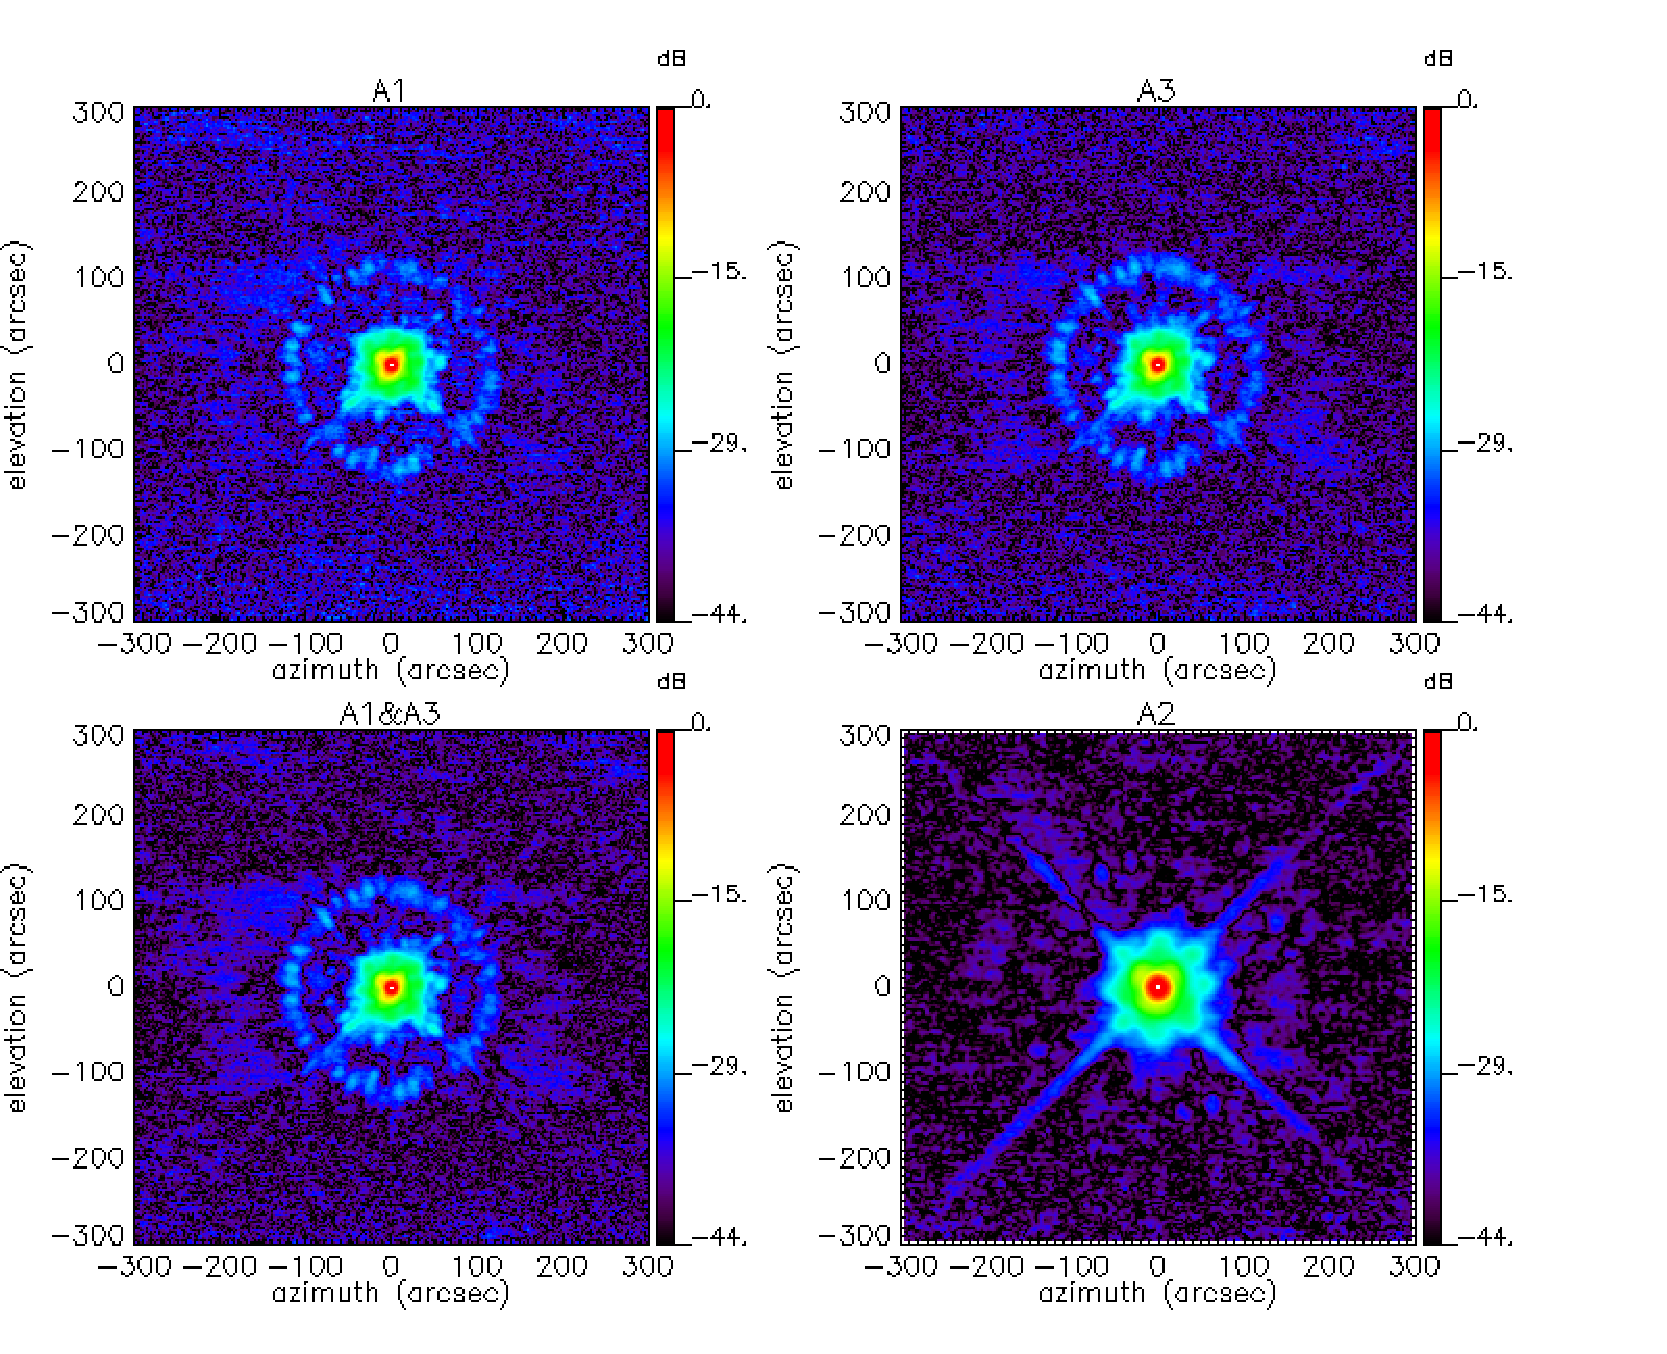
\includegraphics[trim=0cm 0cm 2.5cm 0cm, clip=true, width=\linewidth]{Figures/Lobe_map_Combo_v2_dB.pdf}
% \caption[Beam pattern.]{From upper left to lower right, beam maps of array 1 (labeled 'A1'), array 3 ('A3'), the combination of the $1\,\rm{mm}$ arrays ('A1$\&$3') and the  $2\,\rm{mm}$ array ('A2') are shown in decibel. These maps, which consist of normalized combination of four long OTF scans of bright point sources, are in horizontal coordinates and cover a sky area which extends over 10 arcmin.}
%\label{fig:beam}
%\end{center}
%\end{figure}

\begin{figure}[!thbp]
\begin{center}
  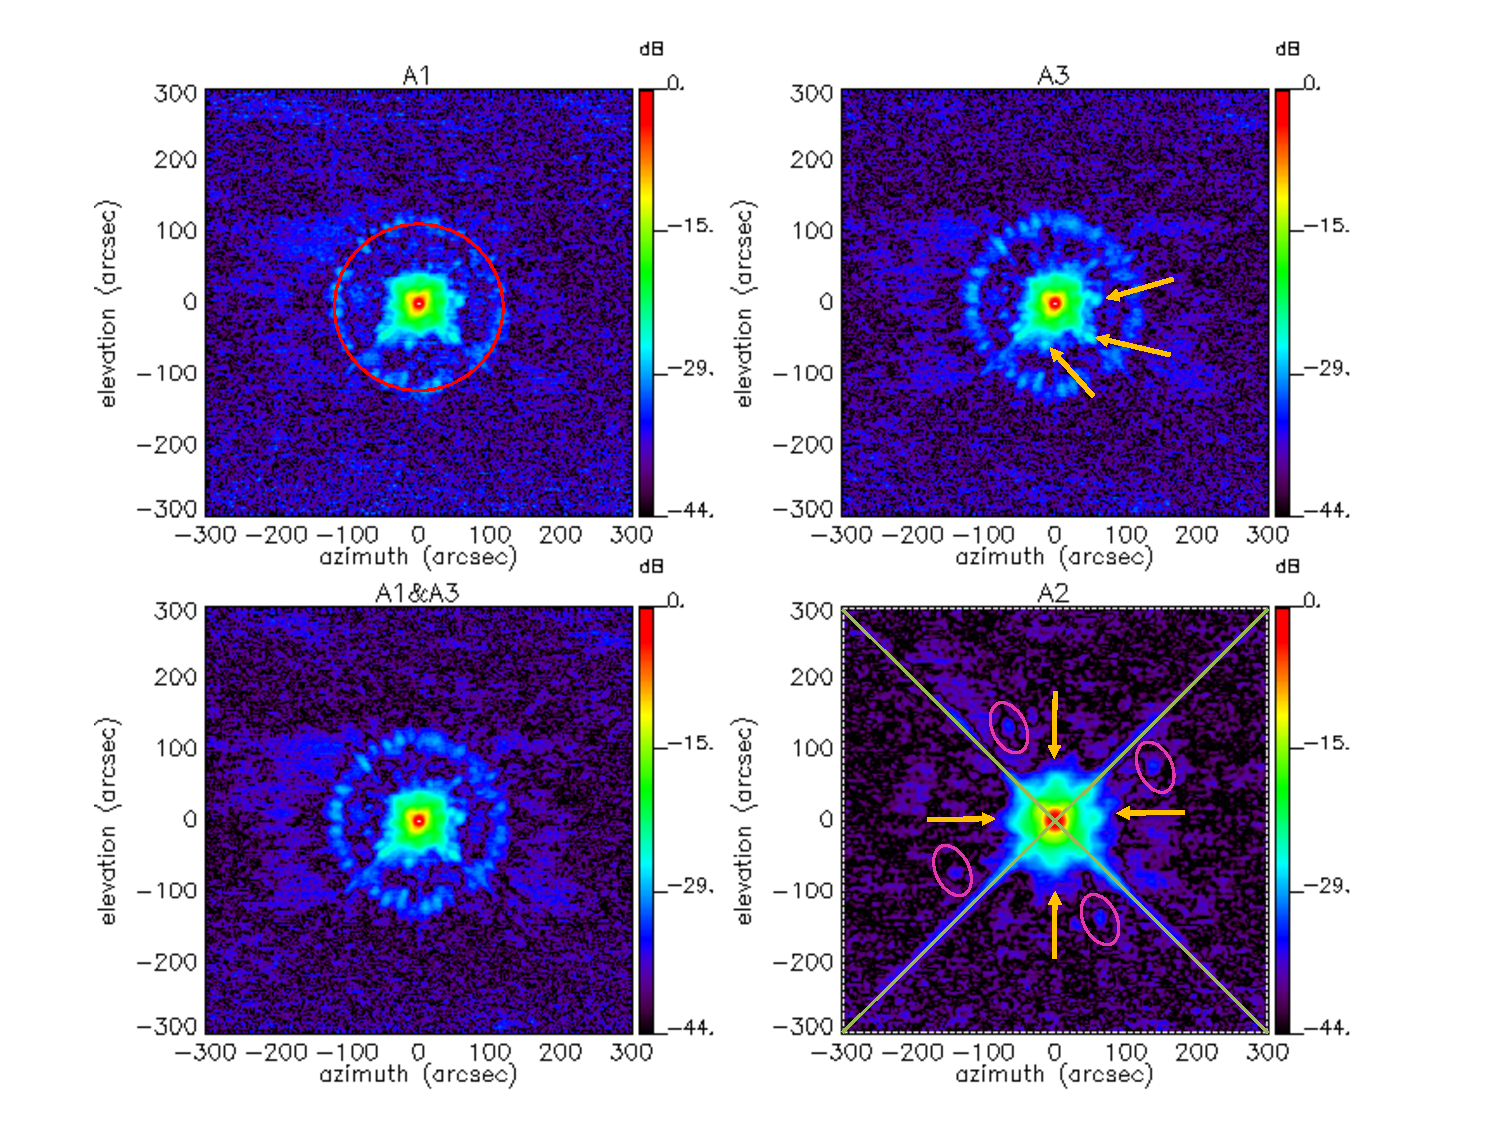
\includegraphics[trim=0.5cm 0.5cm 1cm 0cm, clip=true, width=\linewidth]{Figures/Beams_features.pdf}
\caption[Noticeable features of NIKA2 beam pattern.]{From upper left
  to lower right, beam maps of A1, A3,
  the combination of the $1\,\rm{mm}$ arrays (A1$\&$3) and the
  $2\,\rm{mm}$ array (A2) are shown in decibel. These maps, which
  consist of the normalized combination of four {\tt beammap} scans of
  bright point-like sources, are in horizontal coordinates and cover a
  sky area which extends over $10'$. %Same maps as in Fig.~\ref{fig:beam}
  %with some noticeable features.
  The solid lines and arrows highlight some noticeable features.
  Red circle in the A1 map (upper left panel): diffraction ring seen in 1-mm maps
  (the spokes are presumably caused by radial and azimuthal panel
  buckling \citep{Greve2010}; Orthogonal green lines in the A2 map
  (lower right panel): diffraction
  pattern caused by quadrupod secondary support structure (prominently
  seen in A2 map); Yellow arrows in the A3 map (upper right panel):
  pattern of 3 spikes seen in $1\,\rm{mm}$ maps of unknown origin; Yellow
  arrows in A2 map (lower right panel): four symmetrical spikes of the
  first sidelobes; Pink ellipses: four spikes seen in A2 maps.}
\label{fig:features}
\end{center}
\end{figure}

The NIKA2 beam maps reveal some noticeable features, which are
shown in Fig.~\ref{fig:features}. Ranging from strong and/or extended to
weak and/or spiky, they include:
\begin{enumerate}
\item the main beam and the underlying first error
  beam, which is due to large-scale deformations of the primary
  mirror, and the first side lobes, {\lp which correspond to various diffraction
  patterns. In particular, the 60'' and 85'' diameter (squarish) side
  lobes at $1$ and $2\,\rm{mm}$, respectively, at a level lower than
  $-20\,\rm{dB}$, are due to the convolution of the primary mirror and
  quadrupod diffraction pattern with the pixel (KID) transfer function;}
  %The latter include 
  %the 20" diameter first side lobe and the 60" diameter (squarish)
  %side lobe, which is due to the convolution of the primary mirror and
  %quadrupod diffraction pattern with the pixel (KID) transfer function;
  %The four symmetrical spokes of the error beam as shown by
  %yellow arrows in the A2 panel, are expected from ZEMAX
  %simulations;
   %The 20”/60” “lobes” refer to 1mm or 2mm ? Here, we mixing the terms
  %“error beams” and “side lobes”. Aren’t the 20” diameter “1st side
  %lobe” and the “1st error beam” the same ?  To my understanding, side
  %lobes show up in the maps as rings, e.g. diffraction patterns. Error
  %beams, on the other hand, show-up as broad Gaussians entered on the
  %main beam. The section on the radial averages should take up the
  %discussion of 20” and 60” diameter error beams, and actually show
  %them in the figures.
\item at a much lower level of about $-30\,\rm{dB}$, a diffraction ring shows    
up, which is presumably caused by panel buckling of the primary 
  mirror~\citep{Greve2010}, as shown with a red circle in the A1 panel;
\item also at a level of about $-30\,\rm{dB}$, the side lobes shown with green
  diagonal lines in the A2 panel are due to diffraction on the
  quadrupod holding the secondary mirror of the telescope, as expected
  from ZEMAX simulations;  
\item spikes of not fully understood origin marked by yellow
  arrows. The ones that are along the vertical and
  horizontal axes are reproduced by ZEMAX simulations but at a 
  shallower level, whereas the ones shown in the A3 panel in the
  diagonal directions may be due to the small cylindrical
  instrumentation box on the side of the M2 cabin. The origin of the
  asymmetry on the 1~mm arrays is unknown but most probably due to
  internal optics aberrations;
\item shallow spikes of unknown origin at a level less than $-30\,\rm{dB}$, which are circled by pink
  ellipses. The multiple images on the combined deep beam map indicate
  a rotation of these spikes with the observing elevation, which in
  turn point to diffraction related issue or a ghost image that are
  formed inside the cryostat. These shallow features are expected to
  have no sizable impact on NIKA2 science results.
\end{enumerate}

We further quantify the respective level of the axi-symmetrical
features of the beam pattern by evaluating the beam radial profile
$B(r)$, which is the normalised radial brightness profile,
where $r$ is the radius from the beam center.
%is the azimuthal average of the beam map around the
%main beam center.
Although the profile cannot represent the sub-dominant non-axisymmetrical
features, which are seen in Fig.~\ref{fig:features} (quadrupod
diffraction pattern, spikes), it provides a useful
representation of the internal and central parts of the beam {\lp up to
 about $180''$.} We determine a beam profile from a beam map in centering to
the fitted value of the main beam center and in forming the
weighted average of the map pixels in annular rings.

We checked the stability of the beam against various
observing conditions (source intensity, weather condition, focus
optimisation) by comparing the beam profiles of a series of 18 \bm\
observations.
This set of \bms, which is referred to as {\tt BM18}, has been
selected from all the available \bm\ scans at optimal focus using the
baseline scan selection criteria (Sect.~\ref{se:data_selection}).
%The 18 beam profiles and their difference w.r.t. the median beam
%profile are shown in Fig.~\ref{fig:beam_prof}.
The measured beam profiles using the {\tt BM18} data set are shown in
Fig.~\ref{fig:beam_prof}. {\lp The profiles consist of the main beam and
the first error beams and side lobes, which significantly contribute
at levels of less than $-10\,\rm{dB}$ at both observing
wavelengths. Moreover, at $1\,\rm{mm}$ the contribution of the
diffraction ring, which was marked with a red circle in Fig.~\ref{fig:features},
is seen as a peak at a level up to $-33\,\rm{dB}$ located at a radius
of about $115''$.} Calculating the {\lp rms of the relative}
difference of the beam profiles to the median beam profile, we find a
dispersion below $5\%$ at $1\,\rm{mm}$ and below $2\%$ at
$2\,\rm{mm}$.

{\lp To measure the relative level of the axi-symmetrical beam pattern
features, we further model the beam profiles using an empirical function,
which accounts for the main beam and for a significant fraction of the
error beams and side lobes. This function consists in a three-Gaussian
function $B(r)$ defined as:
\begin{equation}
  B(r) = \sum_{i=1}^{3} \mathcal{A}_i G_i(r) + \mathcal{B}_0,
  \label{eq:3gauss}
\end{equation}
where $\mathcal{A}_i$ is the amplitude of the Gaussian $i$ for
$i \in {1, 2, 3}$ and $\mathcal{B}_0$ a pedestal level accounting for
the residual background level in the map. The measured beam profiles
are fitted using Eq.~\ref{eq:3gauss} and the median best-fit
parameters are given in Table~\ref{tab:mean_3gauss_fit}. The errors
are evaluated as the standard deviation of the best-fitting parameter
values of the 18 \bm\ scans of {\tt BM18}.
These values are given to gain insight of beam profile, but are not
further used for the calibration. We find the level of the first error
beam with respect to the total beam at about $-11\,\rm{dB}$ and
$-13\,\rm{dB}$ at 1 and $2\,\rm{mm}$, respectively.}
%
% AVERAGE 3-GAUSSIAN FIT
\begin{table}[!th]
   \caption{{\lp Median best-fitting values of the parameters of the
  3-Gaussian beam profile, as defined in Eq.~\ref{eq:3gauss}, using
  the {\tt BM18} data set. $\bar{\mathcal{A}_i}$, for
  $i \in {1, 2, 3}$ are the Gaussian amplitudes $\mathcal{A}_i$ relative to the sum
  of $\mathcal{A}_i$, and given in decibel. The FWHM for each of the Gaussian are given in arcseconds.}}
  \label{tab:mean_3gauss_fit}
  \begin{center}
    \begin{tabular}{rll}
      \hline\hline
      \noalign{\smallskip}
%      & \multicolumn{6}{c}{3-Gaussian profile parameters}  \\\cline{1-7}
%      Arrays       & Amp 1 & Amp 2 & Amp 3 & FWHM 1 & FWHM 2 & FWHM      3 \\
       parameters  &  $1\,\rm{mm}$  & $2\,\rm{mm}$ \\
       \noalign{\smallskip} 
      \hline
      \noalign{\smallskip} 
      $\bar{\mathcal{A}_1}$ [dB] &   $-0.33 \pm 0.09$   &  $-0.24 \pm 0.03$ \\
      $\bar{\mathcal{A}_2}$ [dB] &   $-11.4 \pm 1$     &  $-12.8 \pm 0.5$   \\
      $\bar{\mathcal{A}_3}$ [dB] &   $-26 \pm 7$       &  $-27 \pm 3$    \\
      FWHM$_1$  ['']             &   $10.8 \pm 0.2$    &  $17.4 \pm 0.6 $ \\
      FWHM$_2$  ['']             &   $30 \pm 2$        &  $42 \pm 3 $ \\
      FWHM$_3$  ['']             &   $81 \pm 10$       &  $99 \pm 7 $ \\     
%      A1        &  $0.89 \pm 0.01$   &  $0.08 \pm 0.02$  & $5 \times 10^{-3} \pm 2 \times 10^{-3}$  &  $11.0 \pm 0.2 $ & $29 \pm 2 $  & $65 \pm 15 $ \\  
%      A3        &  $0.90 \pm 0.01$   &  $0.07 \pm 0.01$  & $4 \times 10^{-3} \pm 2 \times 10^{-3}$  &  $11.0 \pm 0.2 $ & $30 \pm 3 $  & $72 \pm 23 $ \\  
%      1mm       &  $0.90 \pm 0.01$   &  $0.07 \pm 0.01$  & $4 \times 10^{-3} \pm 2 \times 10^{-3}$  &  $11.0 \pm 0.2 $ & $29 \pm 2 $  & $70 \pm 15 $ \\  
%      2mm       &  $0.96 \pm 0.01$   &  $0.3 \pm 0.3$    & $1 \times 10^{-3} \pm 0.3$ &  $17.5 \pm 0.1 $ & $63 \pm 10 $ & $65 \pm 12 $ \\
       \noalign{\smallskip}   
      \hline
    \end{tabular}    
  \end{center}
\end{table}
%

{\lp For illustration, we show the median best-fit
three-Gaussian profiles at $1$ and $2\,\rm{mm}$ with pink lines, and
the main beam (first Gaussian) profiles with black lines in
Fig.~\ref{fig:beam_prof}. }


%%%%%%%%%%%%%%%%%%%%%%%%%%%%%%%%%%%%%%%%%%%%%%%%%%%%%%%%%%%%%%%%%
% Stability of the beam pattern
\begin{figure}[!thbp]
  \centering
%   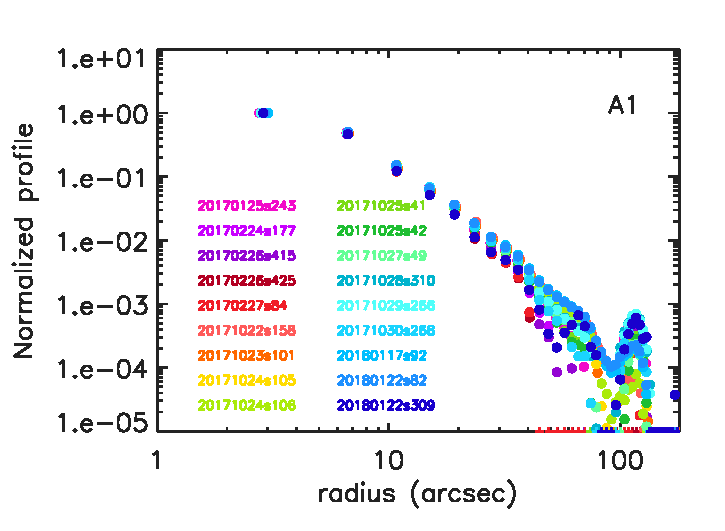
\includegraphics[clip, width=0.42\textwidth]{Figures/Beams/plot_profiles_a1.pdf}
%   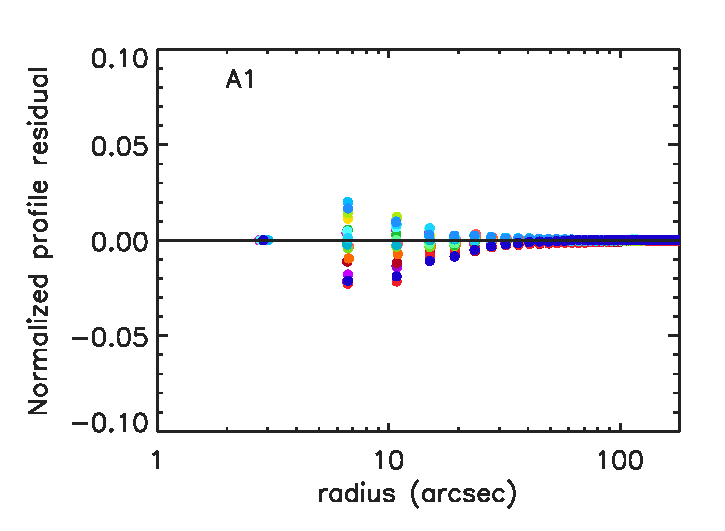
\includegraphics[clip, width=0.42\textwidth]{Figures/Beams/plot_profile_diff_wrt_median_a1.pdf}
%   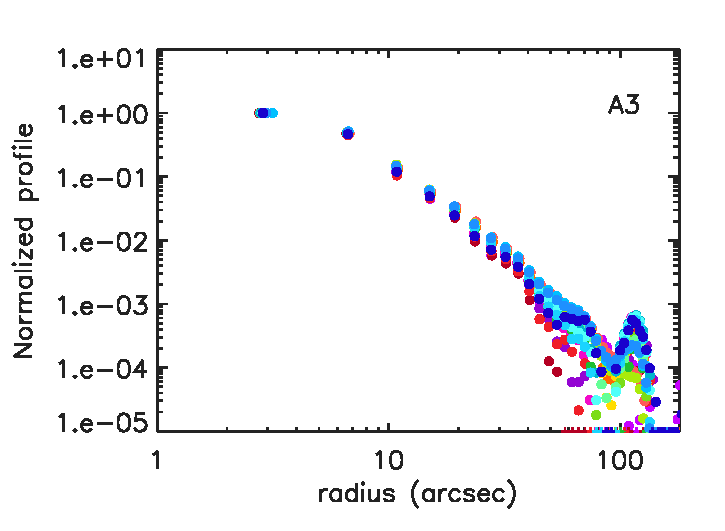
\includegraphics[clip, width=0.42\textwidth]{Figures/Beams/plot_profiles_a3.pdf}
%   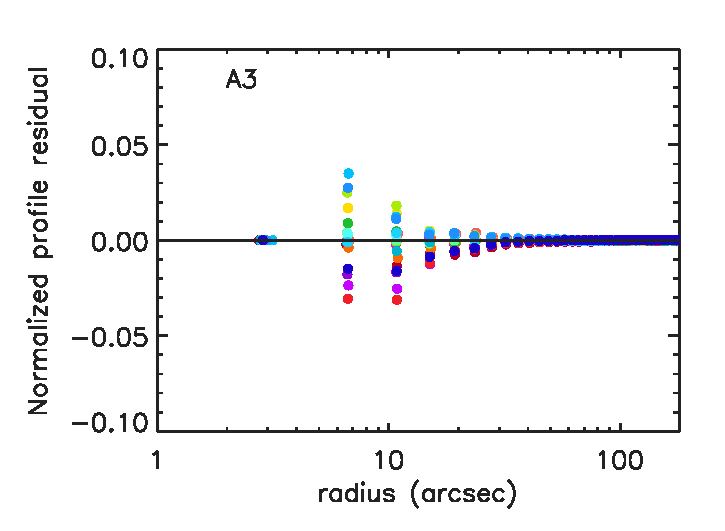
\includegraphics[clip, width=0.42\textwidth]{Figures/Beams/plot_profile_diff_wrt_median_a3.pdf}
   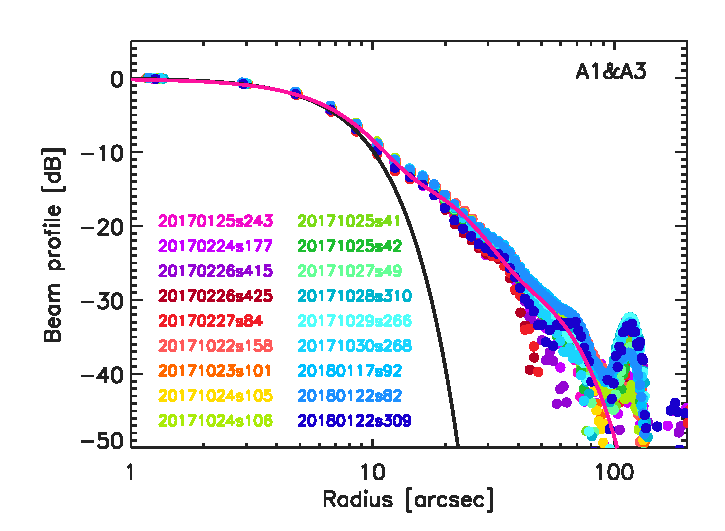
\includegraphics[clip, width=\linewidth]{Figures/plot_profiles_dB_1mm.pdf}
%   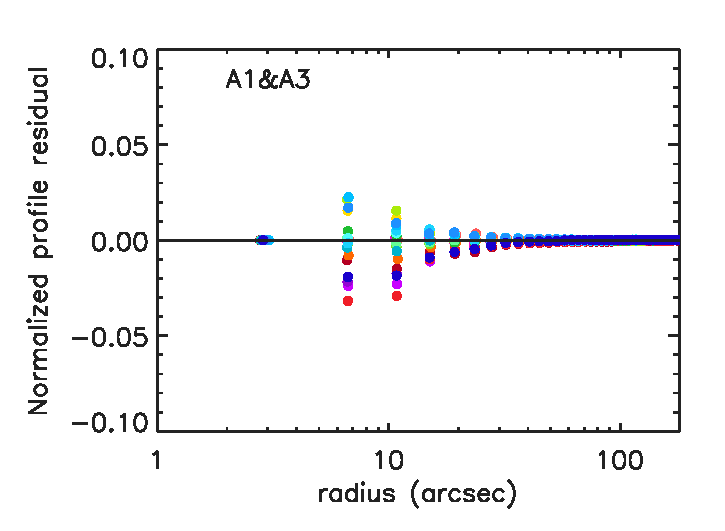
\includegraphics[clip, width=\linewidth]{Figures/plot_profile_diff_wrt_median_1mm.pdf}
   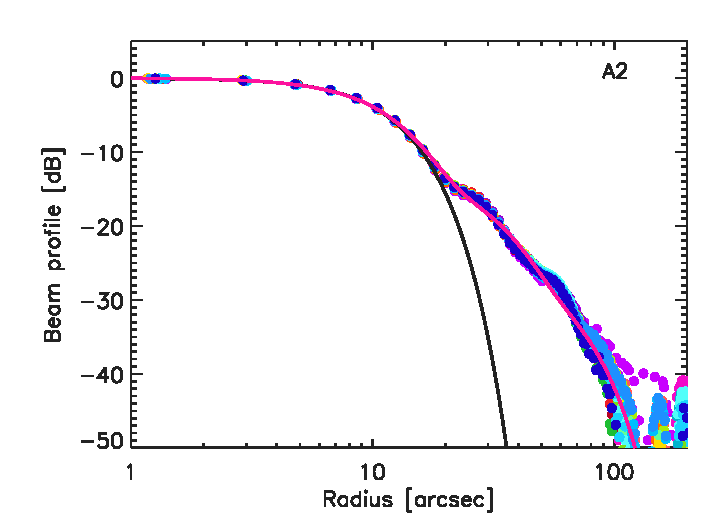
\includegraphics[clip, width=\linewidth]{Figures/plot_profiles_dB_a2.pdf}
%   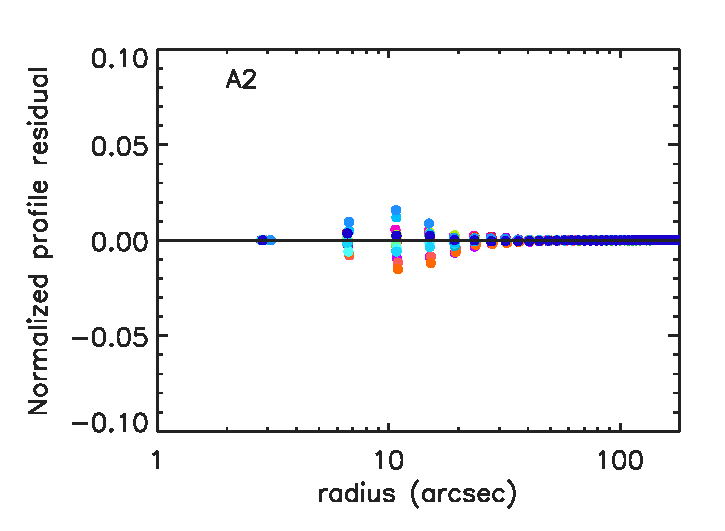
\includegraphics[clip, width=\linewidth]{Figures/plot_profile_diff_wrt_median_a2.pdf}
  \caption[Stability of the beam profile]{{\lp Beam radial
    profiles given in decibel. %as a function of the radius from the
                               %peak, given in dB.
    The data points are the beam profiles for a series of 18
    \bm\ scans acquired during the N2R8 and N2R9 commissioning campaigns and
    during the N2R12 and N2R14 science-purpose campaigns, labeled from the scan
    ID. The black line shows the main beam profile using the combined
    best-fit FWHM, as discussed in Sect.~\ref{se:mainbeam}, while the pink
    line shows the median best-fit three-Gaussian profile, as defined
    in Eq.~\ref{eq:3gauss}.}}
    %Left column plots: 
    %Beam profiles normalised to the maximum value; Right column plots:
    %difference w.r.t. the median normalised profile.
    %The radial
    %profile shapes are stable at better than $5\%$ 
    %against observing conditions.}
  \label{fig:beam_prof}
\end{figure}


%An example of the beam profile from a beam map acquired during {\emph N2R8} (scan ID:
%20170125s243)\todo{verifier le scan utilise pour les figures,
%  possibilite que ce soit 20170125s223 pris l'apres-midi}, as well as the best-fit 3-Gaussian model, is shown in
%the right panels of Fig.~\ref{fig:beam_structure_example}.

%We further fit the three-Gaussian model of Eq.~\ref{eq:3gauss} to each
%profile and gather the average best-fitting amplitudes with respect to
%the peak amplitude and FWHM in Table~\ref{tab:mean_3gauss_fit}. The
%errors are evaluated as the standard deviation of the best-fitting
%parameter values of the 18 \bm\ scans, and thus do not account for the
%correlation between parameters. These values are given to gain insight
%of the axisymmetrical pattern of the beam, but are not further used for
%the calibration. 
%
% AVERAGE 3-GAUSSIAN FIT
%\begin{table}[th]
%  \begin{center}
%    \begin{tabular}{|c|c|c|c|c|c|c|}
%      \hline
%      & \multicolumn{6}{|c|}{3-Gaussian profile parameters}  \\\cline{1-7}
%      Arrays       & Amp 1 & Amp 2 & Amp 3 & FWHM 1 & FWHM 2 & FWHM 3 \\
%      \hline\hline
%      A1        &  $0.89 \pm 0.01$   &  $0.08 \pm 0.02$  & $5 \times 10^{-3} \pm 2 \times 10^{-3}$  &  $11.0 \pm 0.2 $ & $29 \pm 2 $  & $65 \pm 15 $ \\  
%      A3        &  $0.90 \pm 0.01$   &  $0.07 \pm 0.01$  & $4 \times 10^{-3} \pm 2 \times 10^{-3}$  &  $11.0 \pm 0.2 $ & $30 \pm 3 $  & $72 \pm 23 $ \\  
%      1mm       &  $0.90 \pm 0.01$   &  $0.07 \pm 0.01$  & $4 \times 10^{-3} \pm 2 \times 10^{-3}$  &  $11.0 \pm 0.2 $ & $29 \pm 2 $  & $70 \pm 15 $ \\  
%      2mm       &  $0.96 \pm 0.01$   &  $0.3 \pm 0.3$    & $1 \times 10^{-3} \pm 0.3$ &  $17.5 \pm 0.1 $ & $63 \pm 10 $ & $65 \pm 12 $ \\  
%      \hline\hline
%    \end{tabular}
%    \caption[Average 3-Gaussian beam profile parameters]{Average
%      3-Gaussian beam profile parameters. The FWHMs are given in arcseconds.}
%    \label{tab:mean_3gauss_fit}
%  \end{center}
%\end{table}



\subsection{Main beam}
\label{se:mainbeam}

NIKA2 angular resolution {\lp is characterized using the FWHM of a
Gaussian fitted to the main beam. This principal Gaussian encloses
most of the measured flux density of a point-like source.} %However, the
%telescope beam consists of more components, as shown in the previous
%paragraphs.
%We have developped
%three different methods for the NIKA2 main beam characterisation
%, which are detailed
%in Sect.~\ref{se:mainbeam_methods}. Sect.~\ref{se:mainbeam_dataset}
%presents the observing scans that we have selected to derive the results
%discussed in Sect.~\ref{se:mainbeam_results}. We check the stability
%of the FWHM estimate against the observing conditions in
%Sect.~\ref{se:mainbeam_stability}.

\subsubsection{Main beam characterization methods}
\label{se:mainbeam_methods}
To characterize the main beam and to derive an estimate of the FWHM, we
have developed three methods. The two first methods, quoted
{\tt Prof-3G} and {\tt Prof-1G}, rely on a fit of the beam profile to
benefit from the signal-to-noise ratio increase after azimuthally
averaging the signal. The last one by contrast,
consists in an elliptical Gaussian fit of the beam map for a better
2D modeling, and is labeled {\tt Map-1G}. They are presented in more
detail below. \\

\noindent {\tt Prof-3G} consists in fitting the beam profile using the
three-Gaussian function defined in Eq.~\ref{eq:3gauss}.
%, and derive the FWHM from the main beam parameter.
 The main beam FWHM estimate is given by the best-fitting value
of the FWHM for the first Gaussian function. {\lp This main beam FWHM
estimate is expected to be immune to the first error beams
and side lobes, which are well accounted for. For consistency checks,
we also relies on two other methods that rely on simpler beam models.}\\

\noindent {\tt Prof-1G} relies on fitting a single Gaussian to the beam
profile after masking the portion of the profile where the
contributions of the side lobes and error beams are the
largest. Specifically, the side lobe mask is designed to cut out {\lp the
radius ranging from an inner radius
$r_{\rm{in}} = 0.65\, \mathrm{FWHM}_0,$, where FWHM$_0$ is the
reference Gaussian beam FWHM (see Sect.~\ref{se:photometric_system})
to an outer radius $r_{\rm{out}} = 80''$,} centered on the beam
maximum.
%At radial distances
%greater than $80''$, the profile measurement provides the base level
%for the Gaussian fit.
The profile is estimated up to a radius of
$180''$, that is in the inner part of the beam map where the noise
variance is uniform.\\

\noindent {\tt Map-1G} consists in modeling the two-dimensional distribution of
the main beam using an 2D elliptical Gaussian of size $\sigma_x$ and
$\sigma_y$. We characterize NIKA2 main beam using
\begin{equation}
  FWHM = 2 \sqrt{2\ln {2}\, \sigma_x\sigma_y}.
\end{equation}
%where $\sigma_x$ and $\sigma_y$ are the Gaussian standard deviation
%along minor and major axis.
As in {\tt Prof-1G}, we use masked versions of the
beam map to avoid side lobe and error beam contaminations. 
%The mask cuts an annulus of inner radius
%$r_{\rm{in}}$ and outer radius $r_{\rm{out}}$ centered on the beam
%maximum.
Whereas $r_{\rm{out}}$ is conservately set to be $100''$,
$r_{\rm{in}}$ is let free to vary around a central value about $8''$
for A1 and A3 and about $12''$ for A2 to provide the best 2D Gaussian
fit.

\subsubsection{Data sets for the main beam determination}
\label{se:mainbeam_dataset}

We select a sub-set of the selected \bm\ scans described in
Sect.~\ref{se:fullbeam} by discarding scans of Mars. {\lp Indeed, \bms\
toward Mars unveil the complex full beam pattern, which extends beyond
radii of $100''$, so that the annulus sidelobe mask used in {\tt
Prof-1G} and {\tt Map-1G} is not sufficient to mitigate the error
beams and sidelobes effects.}
The 12 remaining \bm\ scans are analysed using the data reduction
pipeline of Sect.~\ref{se:dataproc} and projected onto maps
with a resolution of $1''$ and an angular size of $10'$. This data set
is referred to as {\tt BM12}.

We also consider a series of shorter integration scans. We select
$5' \times 8'$ raster scans of moderately bright to very bright point
sources by thresholding the flux density estimates at $1~\rm{Jy}$ at both
wavelengths. %Slightly extended sources, such as Mars, NGC7027 and
%CRL2688 are discarded.
After the baseline scan selection, as described in
Sect.~\ref{se:data_selection}, the data set comprises 154 %163
scans towards the giant planets Uranus and Neptune, the secondary calibrator
MWC349 and the quasars 3C84, 3C273, 3C345 and 3C454 (aka
2251+158). For these short scans, which are referred to as {\tt
R154}, the data are reduced and projected onto $2''$
resolution maps. 

{\lp Finally, we use a series of 75 observation scans of Uranus and
Neptune, which includes both \bm\ and $5' \times 8'$ raster scans. 
This data set, which is referred to as {\tt UN75}, consists of all the
scans of Uranus and Neptune acquired during the \emph{reference}
observation campaigns (N2R9, N2R12 and N2R14).}


\subsubsection{Results}
\label{se:mainbeam_results}

We have derived the main beam FWHM for the three arrays and the
$1\,\rm{mm}$ arrays combination using the three methods presented in
Sect.~\ref{se:mainbeam_methods} and the data
sets of Sect.~\ref{se:mainbeam_dataset}.
%First, we test the stability of the FWHM estimates against the choices
%of the estimation method by comparing the median FWHM estimate using
%{\tt Prof 1} with the {\tt 2D beam} average FWHM from the 12 \bm\ scan
%sub-set.
Namely, our main beam FWHM estimates
consist of i) the median FWHM estimate using {\tt Prof-3G} on the
{\tt BM12} dataset, ii) the average FWHM estimate using {\tt Prof-1G}
on the {\tt UN75} data set and the {\tt Map-1G} average FWHM using
either {\tt BM12} or {\tt R154}. 
By comparing these results, we test the stability of the FWHM
estimates against the choices of the data set and of the estimation
method. %We also seek at validating the FWHM estimates using
%{\tt Prof 2}, which is further used to derive the beam efficiency in
%Sect.~\ref{se:beam_efficiency}.

In the case of Uranus, the FWHM estimates are further corrected for
the {\lp average beam broadening induced by the extension of the
apparent disc, which is $0.19''$ and $0.12''$ at 1 and $2\,\rm{mm}$,
respectively.}
%At the IRAM $30\,\rm{m}$ latitude,
{\lp During the observation period, Uranus disc diameter has varied
from $3.3''$ to $3.7''$. This diameter variation translates into beam
broadening variations of an amplitude of a few tenth of arcseconds,
which are neglected.}  
%This induces a broadening of the Gaussian main beam of
%$0.19 \pm 0.03\,\rm{arcsec}$ at $1\, \rm{mm}$ and $0.12 \pm 0.02\,\rm{arcsec}$
%at $2\, \rm{mm}$. Uranus FWHM estimates are corrected for the average beam
%widening values.

The results of this analysis are
gathered in Table~\ref{tab:fwhm}, including uncertainties evaluated as
the rms dispersion of single-scan based FWHM estimates.
{\tt Prof-1G} and {\tt Map-1G} results are in agreement within
uncertainties, whereas {\tt Prof-3G} yields slightly smaller FWHM.
%All the tests based on {\tt Prof 2} and {\tt 2D beam}, which both
%resort to a sidelobe mask, yield FWHM estimates
%in agreement within error bars, whereas the test using {\tt Prof 1}
%yields slightly smaller FWHM for all arrays.
%The latter provides us with lower limits for the main beam FWHM.
%The latter constitute optimistic estimates of the FWHM. 
{\lp The latter is more robust againts the error beams and large radii
beam features than the formers, as expected.}
Combined results are obtained from an error-weighted
average of the four FWHM estimates for each array.
Because the rms errors estimated using the 12 \bm\ scans may be
optimistic considering the small statistic, they are conservatively
increased to match the uncertainty estimates based on the {\tt R154}
data set before performing the weighted average.  
%The uncertainties are the most robustly derived from the dispersion of the
%best-fitting FWHM over the set of 154 OTF scans, whereas rms errors
%that are estimated from smaller and more homogeneous scan sets may be
%optimistic. Combined results are obtained from an error-weighted
%average of the four FWHM estimates for each array.
%The 12 \bm\ scan
%based rms errors were replaced by the 154 OTF scan based rms errors
%beforehand.
The combined results, as given in
Table~\ref{tab:fwhm}, provide a robust evaluation of the
FWHM. Hence, we report FWHMs of $11.1'' \pm 0.2''$ at
$1\, \rm{mm}$ and $17.6''\pm 0.1''$ at $2\, \rm{mm}$.  

\begin{table*}[!thbp]
  \caption[]{Estimates of the main beam FWHM in arcsec, using three estimation methods (see
    Sect.~\ref{se:mainbeam_methods}) and three data sets
    (see Sect.~\ref{se:mainbeam_dataset}), and their combination.}
  \label{tab:fwhm}
  \centering
  \begin{tabular}{llrrrr}
    \hline\hline
    \noalign{\smallskip}
    Method   &    Dataset   &  \multicolumn{4}{c}{FWHM ['']} \\
    \noalign{\smallskip}\cline{3-6}\noalign{\smallskip}
        &    &   A1 &  A3 & A1 $\&$ A3 &  A2  \\
    \noalign{\smallskip}
    \hline
    \noalign{\smallskip}
    {\tt Prof-3G}  &  {\tt BM12}    & $10.8 \pm 0.1$  &  $10.8 \pm 0.1$  & $10.8 \pm 0.1$  &  $17.4 \pm 0.1$  \\
    {\tt Prof-1G}  &  {\tt UN75}    & $11.3 \pm 0.4$  &  $11.2 \pm 0.4$  & $11.2 \pm 0.3$   & $17.4 \pm 0.2$  \\ 
    {\tt Map-1G}   &  {\tt R154}    & $11.3 \pm 0.2$  &  $11.1 \pm 0.2$  & $11.2 \pm 0.2$  &  $17.8 \pm 0.1$  \\ 
                   &  {\tt BM12}    & $11.2 \pm 0.1$  &  $11.1 \pm 0.1$  & $11.2 \pm 0.1$  &  $17.6 \pm 0.1$  \\
    \noalign{\smallskip}
    \hline
    \noalign{\smallskip}
    \multicolumn{2}{c}{Combined}               & $11.1 \pm 0.2$  & $11.0 \pm 0.2$  & $11.1 \pm 0.2$  &  $17.6 \pm 0.1$  \\
    \noalign{\smallskip}
    \hline
  \end{tabular}
\end{table*}

\subsubsection{Stability checks}
\label{se:mainbeam_stability}

\begin{figure}[!thbp]
\begin{center}
  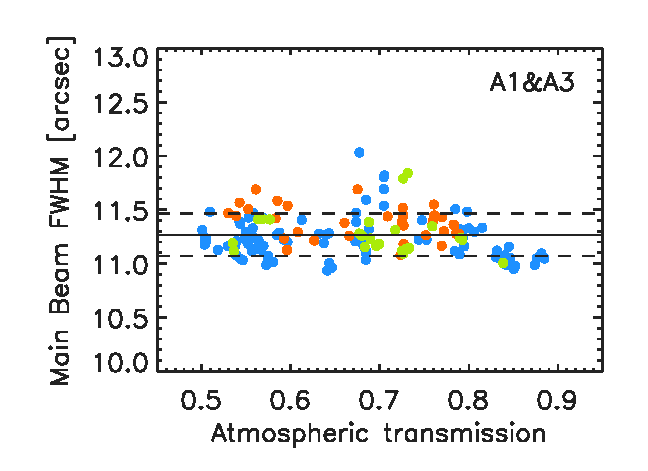
\includegraphics[clip, width=0.4\textwidth]{Figures/plot_FWHM_vs_atmtrans_mb_radius_binning2_1mm.pdf}
  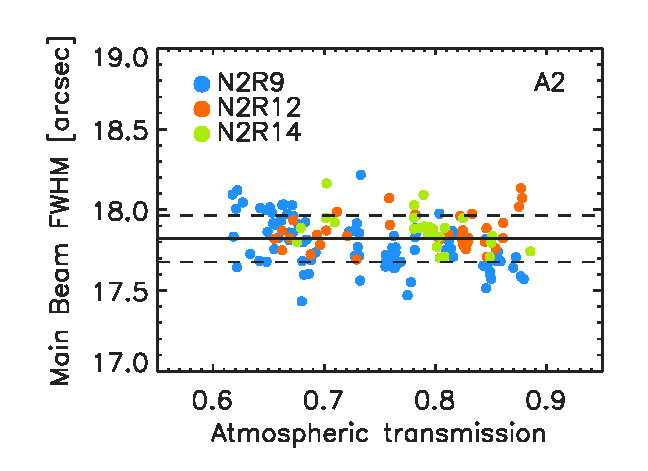
\includegraphics[clip, width=0.4\textwidth]{Figures/plot_FWHM_vs_atmtrans_mb_radius_binning2_a2.pdf}
  \caption[Main Beam FWHM]{Main beam FWHM estimates for the
    $1\,\rm{mm}$ (top) and $2\,\rm{mm}$ (bottom) channels are shown as
    a function of the atmospheric transmission estimated at the
    corresponding wavelengths using bright point source observations
  acquired during the \emph{reference} observation campaings (N2R9, N2R12, N2R14).}
\label{fig:fwhm_map_atmtrans}
\end{center}
\end{figure}

Figure~\ref{fig:fwhm_map_atmtrans} shows the main beam FWHM estimates
using {\tt Map-1G} as a function of atmospheric transmission,
which is modeled as $\exp{\left(-\taunu \ ,x\right)}$. %, where $\tau$
%is the zenith opacity estimate and $x$ the airmass, which is
%evaluated as the cosecant of the observing elevation.
The main beam FWHM estimates using data of the three campaigns are in
agreement within rms errors. Moreover, the main beam FWHM is stable
against atmospheric conditions at both wavelengths. Slightly lower
values than average (about $11''$) are observed in the best
atmospheric conditions at $1\,\rm{mm}$ providing us with a lower limit
in the absence of correlated atmospheric noise residuals. We note
three scans acquired during the N2R12 campaign with larger FWHM than average at
$2\,\rm{mm}$ although the atmospheric transmission was excellent: this
is likely an effect of atmospheric instabilities
%the anomalous refraction
, which affected a large number of observation scans during N2R12. 



\subsection{Beam efficiency}
\label{se:beam_efficiency}

Building upon the description of the full-beam pattern in
Sect.~\ref{se:fullbeam} and the main beam in Sect.~\ref{se:mainbeam},
we derive the beam efficiency for each array, which is defined as the
ratio of the solid angle sustained by the main beam to the total beam
solid angle.

We derive an estimate of the total beam solid angle
\begin{equation}
  \Omega_{\rm{tot}} (A_i, r_{max}) = \int_0^{r_{max}} \frac{B_{A_i}(r)}{B_{A_i}(0)} \,  2 \pi r dr
  \label{eq:omega_tot}
\end{equation}
from the normalised beam profile $B_{A_i}(r)/B_{A_i}(0)$ of the array
$A_i$ integrated up to $r_{max} = 180''$. {\lp Hereafter, we refer to
this total beam solid angle estimate as $\Omega_{180}$.}
The main beam solid angle is
evaluated from the main beam (mb) FWHM, as
$\Omega_{\rm{mb}} = 2 \pi\,  \sigma_{\rm{mb}}^2$, where FWHM$ =
2\sqrt{2\ln{2}}\, \sigma_{\rm{mb}}$. 

The choice of the maximum radius is set both by the integration depth of
the \bm\ scans, which in turn fixes the noise variance, and the
filtering due to the data processing. {\lp As discussed in
Sect.~\ref{se:dataproc}, the latter is actually targeted to the analysis of
point-like or moderately extended sources that are largely encompassed
within a $180''$-radius.}

%A large set of \bm\ scans of Uranus and Neptune acquired during the
%N2R9, N2R12 and N2R14 campaigns have been used to evaluate
%{\lp $\Omega_{180}$} from the measured beam profiles up to
%$r_{max} =180''$. %and $\Omega_{\rm{mb}}$  derived with the main beam FWHM
%estimates using the sidelobe-masked 1D method.
We evaluate {\lp $\Omega_{180}$} from the measured beam profiles
obtained using the {\tt UN75} data set (see Sect.~\ref{se:mainbeam_dataset}).
The result is given in Table~\ref{tab:solid}.

\begin{table}[!h]
\caption{Estimates of the solid angle of the total beam
  $\Omega_{180}$ given in arcsec$^{2}$ using Neptune and Uranus
  scans acquired during three observation campaigns, and the combined
  result. }
\label{tab:solid}
\centering
\begin{tabular}{l cccc}
\hline\hline
\noalign{\smallskip}
Campaigns  & \# scans & %\multicolumn{3}{c}{$\Omega_{\rm{tot}}$ (arcsec$^{2}$)} %& \multicolumn{3}{c}{$\Omega_{\rm{tot}}/\Omega_{gauss}$} \\
%\hline
%     &               &
A1    &    A2   &  A3  \\%& A1  &  A2  & A3   \\
\noalign{\smallskip}
\hline
\noalign{\smallskip}
N2R9     & 27  &  265$\pm$ 23    &  466$\pm$ 17 & 252 $\pm$ 23 \\%&  1.80 $\pm$ 0.12    &  1.35 $\pm$ 0.05   &   1.74 $\pm$ 0.13   \\
N2R12    & 20  &  229$\pm$ 11    &  437$\pm$  9 & 221 $\pm$ 10 \\%&  1.71 $\pm$ 0.06   &  1.30 $\pm$ 0.02   &   1.68 $\pm$ 0.06   \\
N2R14    & 28  &  251$\pm$ 16    &  457$\pm$ 15 & 245 $\pm$ 18 \\%&  1.73 $\pm$ 0.08   &  1.32 $\pm$ 0.03   &   1.72 $\pm$ 0.08   \\
Combined & 75  &  240$\pm$  9    &  446$\pm$  7 & 230 $\pm$  8 \\%&  1.74              &   1.32             &   1.71              \\
\noalign{\smallskip}
\hline
\end{tabular}
\end{table}

Heterodyne observations at the IRAM \trentemetre\ telescope
toward the lunar edge and the measure of forward beam efficiency using
skydips show that a non-neglectible fraction of the full beam stems
from radius greater than $180''$~\citep{Greve1998, Kramer2013}.
An accurate evaluation of the total beam solid angle would require
{\lp the development a dedicated data reduction method tailored to
handled very extended diffuse emission,} as well as a 
dedicated observation program
% to measure of the $4\pi$ integral of the full beam pattern
~\citep{Greve1998, Sugimoto2004, Gusten2006}.
%This fraction is not considered here. Beam efficiency estimators that are based on
%the total solid angle estimates using Eq.~\ref{eq:omega_tot} thus
%overestimates the beam efficiency. An accurate evaluation of
%this quantity would require a dedicated observation program to measure
%of the $4\pi$ integral of the full beam pattern.
{\lp Here we use the IRAM \trentemetre\ telescope beam model described
in \citet{Kramer2013} to evaluate the beam solid angle stemming from a
radius greater than $180''$.
This quantity receives two contributions, the one of the error beams,
which are modeled as three Gaussians, and the one of the forward and
rearward spillover and scattering efficiencies. We compute the solid
angle of the main beam and error beams integrated over a radius ranging
from $180''$ to $390''$, which is the maximum radius covered by \bm\ scan,
$\Omega_{180<r<390}^{\rm{mb+eb}}$, and over radii greater
than $180''$, $\Omega_{>180}^{\rm{mb+eb}}$. The results are given in
Table~\ref{tab:solid_corr}, as well as the contribution of the forward and
rearward spillover and scattering efficiencies to the beam solid angle
$\Omega^{\rm{frss}}$. The total beam solid angle 
$\Omega_{\rm{tot}}$ can be estimated as
\begin{equation}
\Omega_{\rm{tot}} = \Omega_{180} + \Omega_{>180}^{\rm{mb+eb}}
+ \Omega^{\rm{frss}}.
\label{eq:omega_beam_4pi}
\end{equation}

\begin{table}[!h]
\caption{Estimates of the various contribution to the beam solid angle
integrated up to $180''$, up to $390''$ and over $4\pi$ given in
arcsec$^{2}$. }
\label{tab:solid_corr}
\centering
\begin{tabular}{lcc}
\hline\hline
\noalign{\smallskip}
&  A1\&A3 & A2 \\
\noalign{\smallskip}
\hline
\noalign{\smallskip}
$\Omega_{180}$                  &   235 $\pm$  8 & 446 $\pm$  7 \\\noalign{\smallskip}
$\Omega_{180<r<390}^{\rm{mb+eb}}$  &   12          &   20       \\\noalign{\smallskip}
$\Omega_{>180}^{\rm{mb+eb}}$      &   21          &   41      \\\noalign{\smallskip}
$\Omega^{\rm{frss}}$             &   45          &   40      \\
\noalign{\smallskip}
\hline
\end{tabular}
\end{table}
}

We evaluate the main beam efficiencies using both the {\tt UN75} and
the {\tt BM12} data sets, as presented in
Sect.~\ref{se:mainbeam_dataset}. We compare the results based on three
estimates of the total beam and main beam solid angles: 
\begin{itemize}
  \item{{\tt BE1} relies on the best-fitting parameters of the
    three-Gaussian model of the full beam to derive the two solid
    angles. The main beam solid angle thus corresponds to the volume
    enclosed by the first Gaussian, as obtained using {\tt Prof-3G};}
  \item{{\tt BE2} consists in using $\Omega_{180}$ measurements as
    total beam solid angle estimates, while $\Omega_{\rm{mb}}$ is
    derived with the FWHM obtained using {\tt Prof-1G} (see
    Sect.~\ref{se:mainbeam_methods});}
  \item{{\tt BE3} is similar to {\tt BE2} but the main beam FWHM is
    derived using {\tt Map-1G}.}  
\end{itemize}

The beam efficiency estimates using the three methods are gathered
in Table~\ref{tab:beam_efficiency}: central values and error
bars are evaluated as the median and the rms error of the
estimates on individual \bms\ respectively. A robust evaluation of the
beam efficiency uncertainties is obtained using the rms error estimates
for {\tt BE2}, which are based on 75 \bm\ scans. We combined the
results of the three methods using an error-weighted average. Rms
errors of {\tt BE1$\&$BE3}, which rely on 12 scans, are conservatively
increased to be at least equal to {\tt BE2} rms errors beforehands.
%By contrast, error
%estimates for {\tt BE1$\&$BE3} rely on 12 scans and are thus less
%robust. We combined the results of the three methods using an error-weighted
%average. {\tt BE2} rms errors are conservatively used as a lower
%limit of the error estimates for all methods.

Using the combined results, as given in
Table~\ref{tab:beam_efficiency}, we report beam efficiencies of
$55 \pm 3 \%$ at $1\,\rm{mm}$ and  $77 \pm 2 \%$ at $2\,\rm{mm}$. 
  
%res1 = [0.54, 0.54, 0.53, 0.74]
%res2 = [0.55, 0.56, 0.55, 0.76]
%res3 = [0.59, 0.58, 0.59, 0.80]
%res = [[res1], [res2], [res3]]
%s1 = [0.03, 0.04, 0.03, 0.04]
%s2 = [0.03, 0.03, 0.03, 0.02]
%s3 = [0.07, 0.04, 0.04, 0.02]
%sig = [[s1], [s2], [s3]]
%for i = 0, 3 do print, total(res[i, *]/sig[i, *]^2)/ total(1d0/sig[i, *]^2)
%for i = 0, 3 do print, sqrt(1d0/ total(1d0/sig[i, *]^2))

\begin{table}[!h]
  \caption[]{Main beam efficiencies given in percent.}
  \label{tab:beam_efficiency}
  \centering
  \begin{tabular}{l cccc}
    \hline\hline
    \noalign{\smallskip}
    %
    %&    \multicolumn{4}{c}{Array or array combination} \\
    %\cline{2-5}
    Method & A1 &  A3 & A1 $\&$ A3 &  A2  \\
    \noalign{\smallskip}
    \hline
    \noalign{\smallskip}
    {\tt BE1}  &  $54 \pm 3$  & $54 \pm 4$  &  $53 \pm 3$  &  $74 \pm 4$  \\
    {\tt BE2} &  $55 \pm 3$  & $56 \pm 3$  &  $55 \pm 3$  &  $76 \pm 2$  \\
    {\tt BE3}&  $59 \pm 7$  & $58 \pm 4$  &  $59 \pm 4$  &  $80 \pm 1$  \\
    combined          &  $55 \pm 3$  & $56 \pm 3$  &  $55 \pm 3$  &  $77 \pm 2$  \\
    \noalign{\smallskip}
    \hline
  \end{tabular}
  %\tablefoot{ \\
  %  \tablefoottext{a}{based on {\tt Prof 3G} best-fitting parameters}
  %  \tablefoottext{b}{based on {\tt Prof 1G} main beam FWHM} 
  %  \tablefoottext{c}{based on {\tt Map 1G} main beam FWHM} 
 % }
\end{table}

%We note a
%mild improvement of the beam efficiency between the N2R9 campaign and
%the following campaigns. This could be due to the change of the method
% of setting the telescope focus:  while the focus was set at the
%best value for the center the arrays during N2R9, from N2R12
%on, the focus is set to the optimal value across the array (see the
%discussion in Sect.~\ref{}).    

\begin{table}[!ht]
\caption{Main beam efficiency estimates per observation campaigns,
given in percent.}
\label{tab:MB}
\centering
\begin{tabular}{lcccc}
\hline\hline
\noalign{\smallskip}
campaign &  A1    &    A2   &  A3    \\
\noalign{\smallskip}
\hline
\noalign{\smallskip}
N2R9    &  54.1$\pm$ 3.2   &  74.7$\pm$ 2.9  & 55.9 $\pm$ 3.7      \\
N2R12   &  55.7$\pm$ 2.0   &  77.4$\pm$ 1.0  & 57.1 $\pm$ 2.0      \\
N2R14   &  55.0$\pm$ 2.7   &  76.0$\pm$ 1.8  & 56.1 $\pm$ 2.6     \\
            %\noalign{\smallskip}
            \hline
\end{tabular}
\end{table}

As a stability check of the beam efficiency, we detail the {\tt BE2} estimates
%, as well as the level of the error beam,
for each observation campaigns, as given in Table
\ref{tab:MB}. %The level of the error beam is given relative to the
%main beam peak.%(we recall that -12dB as found is $6\%$).
We find stable beam efficiencies using observations acquired one year apart.

%\begin{table*}[!h]
%\caption{Main beam efficiency and level of error beam}
%\label{tab:MB}
%\centering
%\begin{tabular}{l| c | c c c | c c c}
%\hline\hline
%\noalign{\smallskip}
%run  & Nber of scans & \multicolumn{3}{|c|}{Main beam efficiency ($\%$)} & \multicolumn{3}{c}{Error beam level (dB)} \\
%\hline
%     &               &  A1    &    A2   &  A3    & A1  &  A2  & A3   \\
%            \hline
%N2R9    & 27  &  54.1$\pm$ 3.2   &  74.7$\pm$ 2.9  & 55.9 $\pm$ 3.7   &  -11.5 $\pm$ 0.8    &  -14.9 $\pm$ 0.6   &  -12.0 $\pm$ 0.6   \\
%N2R12   & 20  &  55.7$\pm$ 2.0   &  77.4$\pm$ 1.0  & 57.1 $\pm$ 2.0   &  -13.4 $\pm$ 0.3    &  -16.1 $\pm$ 0.3   &  -13.8 $\pm$ 0.3   \\
%N2R14   & 28  &  55.0$\pm$ 2.7   &  76.0$\pm$ 1.8  & 56.1 $\pm$ 2.6   &  -12.5 $\pm$ 0.6    &  -15.3 $\pm$ 0.6   &  -12.7 $\pm$ 0.8   \\
%            %\noalign{\smallskip}
%            \hline\hline
%\end{tabular}
%\end{table*}

